\documentclass{llncs}
\usepackage{tabu}
\usepackage{graphicx}
\usepackage[utf8]{inputenc}

\begin{document}

\title{EM Side-Channel Analysis of ECC Scalar Multiplication}
\author{Sebastian Verschoor, Alvin Cai Kunming}
\institute{Technische Universiteit Eindhoven, Eindhoven, The Netherlands}
\maketitle
%
\begin{abstract}
The aim of the project is to successfully run an electromagnetic side channel attack on the Lim-Lee ECC scalar multiplication algorithm implemented on a smart card. 
\end{abstract} 
%
\section{Introduction}

The electric current that flows through a conductor induces Electromagnetic (EM) emanations which can be used for side channel analysis. The advantage of this technique is that it (a) allows the measurement of local EM radiations from selected points on the chip \cite{gandolfi2001} and (b) attacks can be mounted from a distance of several feet away \cite{kenworthy2012} e.g. against mobile devices.

In this paper, we attempt a practical attack on a smartcard performing ECC scalar multiplication using EM analysis. This attack targets the Lim-Lee scalar multiplication algorithm on Riscure's training card 8. In this report, we will not go into details of the Lim-Lee algorithm and associated attack, but will focus instead on the EM aspects which can be generalised to any scalar multiplication algorithm.

\section{Methodology and Practical Results}

In our attack, we first try to identify the specific location where cryptographic operations are carried out on the smartcard. We can then position the EM probe very close to this region so as to increase the chances of capturing data-dependent signals. The EM traces we obtained were very noisy and required signal processing to reduce noise to levels at which the data dependencies are revealed. The final step is to perform a simple side channel analysis to recover the secret key bits.

\subsection{Spatial Positioning}

\begin{enumerate}
  \item  setup\ldots 
  \item how to identify 30.8MHz crypto core frequency from the power trace (challenging also because there were other strange frequencies ( 7.7 MHz, 15.35MHz, 38.36 MHz)
  \item how to find this point on the chip. 
  \item How we efficiently to iteratively measure and narrow down the region.
\end{enumerate}


\subsection{Signal Processing}

The first step in the signal processing was to isolate the information bearing signal. The most straightforward step was hence to remove the 4MHz signal and its harmonics that arise from the main processor. The 30.8 GHz signal we are interested in is preserved as shown in Figure \ref{figure:harmonics_removal}.

    \begin{figure*}
      \centering
      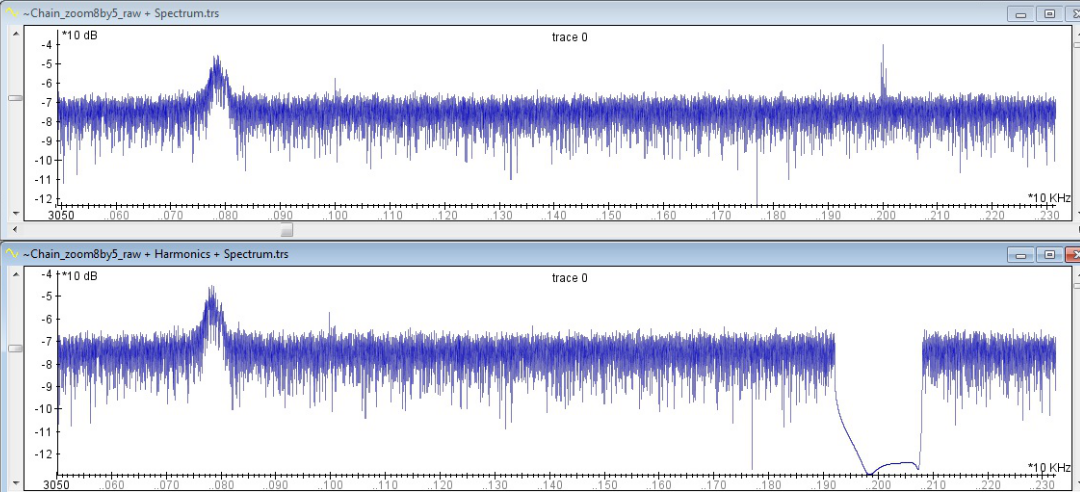
\includegraphics[scale=0.3]{img/harmonics_removal.png}
      \caption{\label{figure:harmonics_removal}Removal of 4GHz harmonics.}
    \end{figure*}  

The EM signal was sampled at a very high frequency (250 Mhz to 1 GHz), and fluctuates frequently between positive and negative values. To better analyse the signal, we try to obtain the absolute value of the signal envelope by using the ``Sync Resample" module which  resamples the original signal at a 30.8 MHz sample rate. Thereafter, we perform low pass filtering. 

These three steps were sufficient to produce a sufficiently clear signal for simple side channel analysis. In the Lim-Lee algorithm, a single scalar multiplication has many rounds. At the beginning of each round, we observe a distinct pattern of 5 or 7 bumps as shown in Figure \ref{figure:pattern}. Here, 5 bumps indicate a 0-bit and 7 bumps indicates a 1-bit value of the nonces used in Lim-Lee. Sufficient nonce values can be obtained across approximately 50 traces (using different input points) to recreate the secret ECC scalar.

Although these three signal processing steps were sufficient, we could additionally have averaged multiple EM traces (using the same  input Point) to produce an even clearer signal, for each of the required 50 traces.

    \begin{figure*}
      \centering
      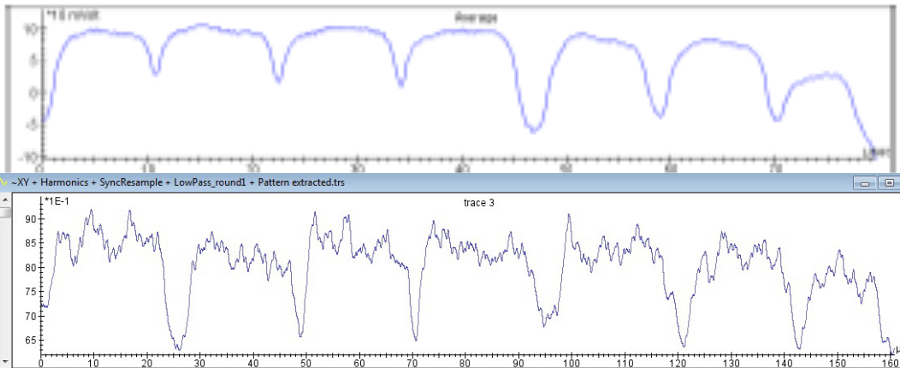
\includegraphics[scale=0.3]{img/pattern.png}
      \caption{\label{figure:pattern}The upper image was obtained from an unfiltered power trace. The lower image was our actual EM measurements after signal processing.}
    \end{figure*}  






\subsection{Simple Side Channel Analysis}
\begin{enumerate}
  \item just provide a brief description as anyway we did not do this completely. 
  \item I think its more interesting to talk about how we can perform a proper attack given the limitations (i.e. can only measure short sections each time.)
  \item \ldots
\end{enumerate}





\section{Conclusion}

\begin{enumerate}
  \item Talk about how practical?
\end{enumerate}

% Add entries in the bibliography that aren't cited:
% \nocite{gandolfi2001}
% \nocite{kenworthy2012}

\bibliographystyle{splncs03}
\bibliography{literature}
% \begin{thebibliography}{99}
% 
% \bibitem{Gandolfi}
% Gandolfi, Karine, Christophe Mourtel, and Francis Olivier. "Electromagnetic analysis: Concrete results." Cryptographic Hardware and Embedded Systems—CHES 2001. Springer Berlin Heidelberg, 2001.
% 
% \bibitem{cri}
% Gary Kenworthy and Pankaj Rohatgi. "Mobile Device Security: The case for side channel resistance." Cryptography Research Inc, 2012.
% 
% 
% \end{thebibliography}
\end{document}
